% Status: draft

\section{Introduction to Jolie}

Jolie is a service-oriented programming language, and is build to support a
microservice natively. In this section we will cover what kind of language
Jolie is, and how it is currently used.

Jolie has a C-inspired syntax, and is dynamically typed. Its interpreter is
written in Java.

The language has no native functions or methods, but instead works in
processes. A process has no arguments, and does not contain any stack (in the
case of recursive calls). There are two pre-defined processes, which will
always be called by the interpreter, these are called \verb!init! and
\verb!main!.

\begin{listing}[H]
\begin{minted}{jolie}
include "console.iol"

define PrintOutput {
    println@Console(output)() // Prints 'OK'
}

init { a = 1 }

main {
    b = 2;
    c = a + b; // c = 3
    if (c == 3) {
        output = "OK"
    } else {
        output = "Bad"
    };
    PrintOutput // Calls the defined process 'PrintOutput'
}
\end{minted}
\caption{A very simple Jolie program}
\label{lst:simple_jolie}
\end{listing}

Listing \ref{lst:simple_jolie} shows a very simple programming language, in
what looks like what you might expect from a dynamic language with C-inspired
syntax. However a few things may also strike you as odd.

First of all there are typos on lines 12, 14 or 16, the semicolon is not needed
here, in fact it would be a syntax error. The reason for this is that the
semicolon isn't used strictly for parsing purposes, but it instead for having
multiple statements in a process. The "semicolon" statement, also called a
sequence statement, has a syntax of \verb!A ; B!, which should be read as:
first perform statement \verb!A!, then perform \verb!B!. The sequence
statement requires both of the operands to be present, hence the syntax error.
Another similar statement is the parallel statement, which has a syntax of
\verb!A | B!, which reads as: do \verb!A! and \verb!B! in parallel. Using
these operators together allows the programmer to easily create a fork-join
workflow. This is typically used in microservices when we want to collect
data in parallel, and continue once all of the data has been retrieved.

Secondly has slightly different rules for scoping. In Jolie everything not
defined in the global scope goes into the same scope. This also persists
through calls to defines. This is the reason that \verb!PrintOutput! can use
the output variable.

Several execution modes exists. The default execution mode, which was used in
Listing \ref{lst:simple_jolie} is \verb!single!. This means that the
\verb!main!  process is run just a single time. Two more modes exists, those
being \verb!concurrent! and \verb!sequential!. TODO Some more stuff

Ports are the primitive that Jolie uses for communication, two types of ports
exists: input and output. Ports describe a running service, where it is located
(\verb!Location!), and how to speak to it (\verb!Protocol!), and finally which
operations it supports (\verb!Interfaces!). In Listing \ref{lst:simple_port} we
see a simple output port which contacts \verb!example.com! on port 42000, using
\verb!http!. Note that it is only the ports that deal with the protocol,
everything inside of the code is completely agnostic with respect to the
protocol being used for communication. As a result it is easy to change a
service from communicating using one protocol to another.

\begin{listing}[H]
\begin{minted}{jolie}
outputPort Example {
    Location: "socket://example.com:42000"
    Protocol: http
    Interfaces: IExample
}
\end{minted}
\caption{A simple output port which contacts the Google website}
\label{lst:simple_port}
\end{listing}

The interface which the port uses is called \verb!IExample!, a full definition
of it can be seen in Listing \ref{lst:simple_interface}. Two types of
operations exists in Jolie, namely \verb!RequestResponse! and \verb!OneWay!.
The difference being fairly self-explanatory, the first receives a request and
returns a response, the other simply receives a request, and produces no
response.

\begin{listing}[H]
\begin{minted}{jolie}
interface IExample {
    RequestResponse:
        anOperation(RequestType)(ResponseType)

    OneWay:
        hello(HelloType)
}
\end{minted}
\caption{An interface in Jolie defines which operations a port exposes}
\label{lst:simple_interface}
\end{listing}

Whenever the Jolie interpreter invokes an operation on an output port, or
receives a request on an input port, the types will be checked. This check
ensures that we don't send out incorrect requests, and ensures that we do not
attempt to process an incorrect request. Listing \ref{lst:simple_types} show
the request and response type of \verb!anOperation!.

\begin{listing}[H]
\begin{minted}{jolie}
type RequestType: void {
    .a: int
    .b: string
    .c: bool
    .d: double
    .e: any // any primitive type
}

type ResponseType: int {
    .aFixedArray[1, 3]: string
    .aNonFixedArray[0, *]: string
    .fieldWithChildren: void {
        .a: void {
            .b: int
        }
    }
}
\end{minted}
\caption{Jolie types are tree-like structures}
\label{lst:simple_types}
\end{listing}

In Jolie types are tree-like structures, very similar to how, for example, XML
would be represented. Importantly the root may also contain a value, this is
different from how most other programming languages work. This also means that
certain encodings may have problems with this. JSON a popular format for
serialization does not support root values, as a result Jolie will encode the
root value under a special key to work around this fact.

TODO Actually use this illustration for something, should probably work with
the actual example provided.

\begin{listing}[H]
\begin{minted}{text}
                         +----------+
                         |          |
                         +----------+
                              /\
                             /  \
                            /    \
                           /      \
                    +------+      +-------+
                    |      |      |       |
                    +------+      +-------+
                     /  |  \
                    /   |   \
                   /    |    \
                  /     |     \
          +-------+ +------+ +--------+
          |       | |      | |        |
          +-------+ +------+ +--------+
\end{minted}
\end{listing}

Jolie natively supports a variety of techniques for composition of services.
The most important (for this work), which we will cover here are
\textbf{aggregation} and \textbf{embedding}.

Embedding allows for a larger service to run smaller services as inner
components. These services communicate with each other using more efficient
local communication. These embedded services can be other Jolie services, but
may also be services written in, for example, Java or even JavaScript.
Communicating with these services is done exactly the same way as with any
other service, it is entirely transparent to the application code where the
service is located. TODO Can probably say a few more words about this subject.
Might be easier to add this later when we know what we actually need.

Aggregation is a generalisation of proxies and load balancers. An illustration
of this concept can be seen in Figure \ref{fig:aggregation}. Aggregation is
useful for creating a wide variety of proxy like architectural patterns. The
aggregation feature is often used along side the courier and interface extender
features. Couriers allows the developer to insert code in-between the receiving
the request and forwarding it. These features for example allow you to add
authentication to a service which otherwise doesn't have it. This is done
entirely without having to touch the original service.

\begin{figure}[H]
    \centering
    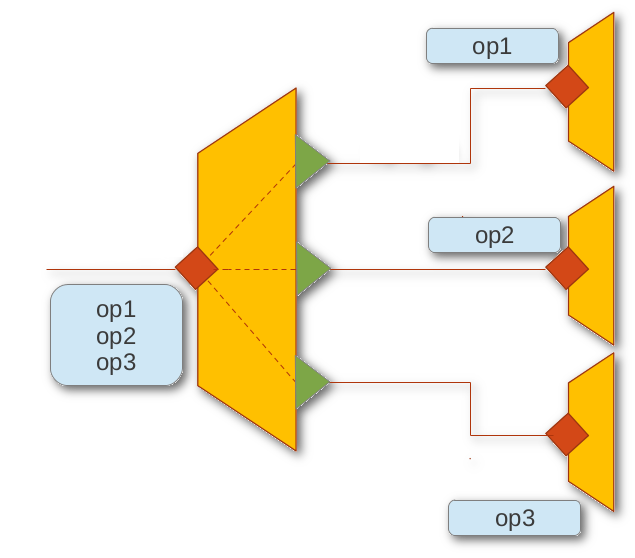
\includegraphics[width=0.6\textwidth]{pictures/aggregation.png}
    \caption{Aggregation is a generalisation of proxies and load balancers}
    \label{fig:aggregation}
\end{figure}

